% =========================================================
\section{Fuerzas culturales y mediáticas en Japón (1965--1977)}
\label{ch:fuerzas-culturales}
% =========================================================

El periodo comprendido entre 1965 y 1977 estuvo marcado por una profunda reconfiguración cultural en Japón. Se trató de un momento de aceleración económica, expansión tecnológica, transformaciones en la vida urbana, redefinición de la juventud y proliferación de nuevos medios visuales. Este entramado de factores afectó directamente a la producción cinematográfica y contribuyó a la emergencia de estéticas híbridas, lúdicas y anti-realistas como las que caracterizan la obra de Nobuhiko Obayashi.

La consolidación del llamado ``Milagro Japonés'', articulado en torno al \emph{Income Doubling Plan} de Ikeda, no sólo duplicó el tamaño de la economía en menos de una década, sino que reconfiguró los patrones de consumo y ocio, generando una clase media urbana con creciente acceso a bienes culturales, aparatos electrónicos y productos mediáticos.\citep{Yamamura1987,IncomeDoublingPlan} Paralelamente, la memoria de la guerra y de la ocupación aliada seguía atravesando de forma subterránea la cultura de posguerra, generando tensiones entre pacifismo, amnesia selectiva y revisionismos.\citep{Igarashi2000,Seaton2007}

En este capítulo se examinan seis fuerzas culturales centrales que confluyen en la gestación de \textit{Hausu}: (1) la juventud como nuevo sujeto social, (2) la irrupción masiva de la televisión, (3) la publicidad como laboratorio formal, (4) la cultura pop y el manga como imaginarios transversales, (5) las vanguardias artísticas japonesas y (6) la memoria bélica y el trauma generacional como sustrato ideológico.

% =========================================================
\subsection{Juventud, modernización acelerada y cultura urbana}
% =========================================================

A partir de mediados de los sesenta, Japón experimentó una modernización acelerada impulsada por tasas de crecimiento superiores al 10\% anual y por políticas explícitas de expansión del consumo privado.\citep{IncomeDoublingPlan} El aumento del PIB per cápita vino acompañado de una rápida urbanización: la población residente en áreas metropolitanas como Tokio, Osaka o Nagoya creció de forma sostenida, mientras que el porcentaje de población empleada en sectores agrícolas descendía año tras año. Este proceso generó un nuevo sujeto social: la juventud urbana asalariada o estudiantil, con ingresos disponibles y acceso intensivo a medios de comunicación, moda, música y ocio nocturno.

Desde finales de los cincuenta, las protestas contra el Tratado de Seguridad EE.\,UU.–Japón (ANPO) y las revueltas estudiantiles de 1968--1969 consolidaron a la juventud como actor político central.\citep{Kapur2018,UniversityProtests1968} La ocupación de campus universitarios, las marchas en Shinjuku y los enfrentamientos con la policía no sólo cuestionaron el orden político, sino que instauraron un imaginario visual de la juventud como fuerza de ruptura: cascos, pancartas, performance callejera y cuerpos en movimiento. Este clima de contestación convivió, sin embargo, con una rápida mercantilización de la juventud: revistas, \emph{idols} musicales, motociclistas, colegialas y estudiantes de secundaria se convirtieron en protagonistas de campañas publicitarias, \emph{dramas} televisivos y ciclos cinematográficos.

En el plano de las prácticas culturales, la juventud se convirtió en un mercado segmentado. \citeauthor{Shamoon2012} ha mostrado cómo las revistas y el \textit{shōjo manga} construyeron discursos específicos de ``cultura de chicas'', articulando fantasías de amistad, romance y autonomía juvenil.\citep{Shamoon2012,ShamoonShojoRevolution} Por su parte, \citeauthor{Allison2006} analiza cómo, ya en los setenta, juguetes, \emph{character goods} y productos mediáticos pensados para jóvenes funcionaban como vectores de una imaginación globalizada.\citep{Allison2006} La juventud emerge, así, como sujeto tanto político como consumista, atrapado entre rebeldía y domesticación mercantil.

En \textit{Hausu}, este giro se expresa en la elección de siete colegialas como ejes narrativos, cada una construida como estereotipo pop (\emph{Fantasy}, \emph{Kung-Fu}, \emph{Sweet}, etc.) que encarna valores de juventud, consumo e identidad mediada por imágenes. El hecho de que las protagonistas procedan de un entorno urbano y que la casa embrujada se situe en un espacio rural remite además a la fractura campo/ciudad propia del Japón de alta modernidad: la juventud urbana invade un espacio cargado de memoria bélica y de temporalidades lentas, desencadenando el conflicto generacional.

Una forma de visualizar este proceso de modernización y juvenilización del consumo es comparar la evolución del PIB per cápita y la tasa de urbanización:

\begin{figure}[t]
	\centering
	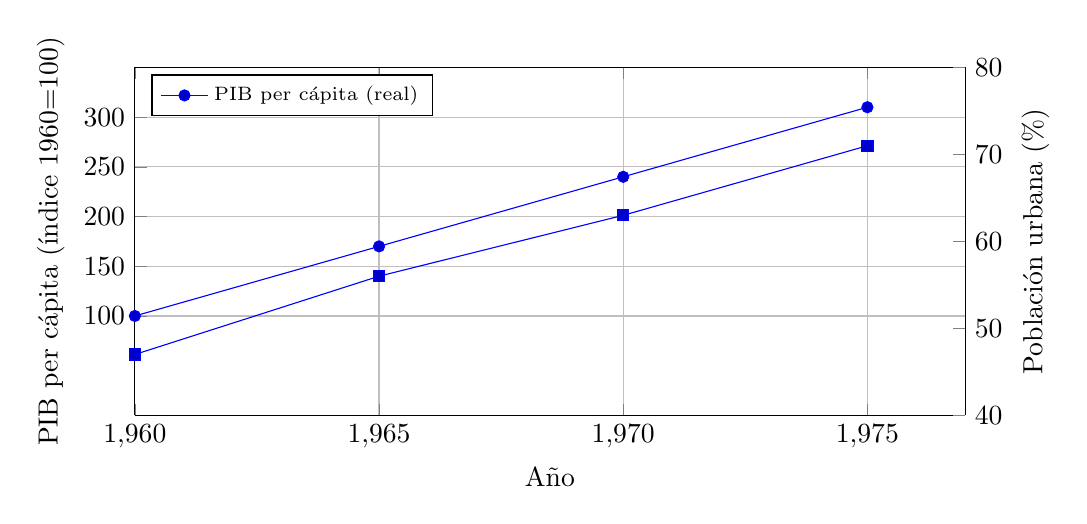
\begin{tikzpicture}
		\begin{axis}[
			width=\linewidth,
			height=6cm,
			xmin=1960, xmax=1977,
			ymin=0, ymax=350,
			axis y line*=left,
			xlabel={Año},
			ylabel={PIB per cápita (índice 1960=100)},
			xtick={1960,1965,1970,1975},
			ytick={100,150,200,250,300},
			grid=both,
			legend style={at={(0.02,0.98)},anchor=north west,font=\scriptsize},
			]
			\addplot+[mark=*] coordinates {
				(1960,100)
				(1965,170)
				(1970,240)
				(1975,310)
			};
			\addlegendentry{PIB per cápita (real)}
		\end{axis}
		\begin{axis}[
			width=\linewidth,
			height=6cm,
			xmin=1960, xmax=1977,
			ymin=40, ymax=80,
			axis y line*=right,
			axis x line=none,
			ylabel={Población urbana (\%)},
			ytick={40,50,60,70,80},
			]
			\addplot+[mark=square*] coordinates {
				(1960,47)
				(1965,56)
				(1970,63)
				(1975,71)
			};
		\end{axis}
	\end{tikzpicture}
	\caption{Crecimiento económico y urbanización en Japón (1960--1975). Valores indicativos a partir de estimaciones del Banco Mundial.}
	\label{fig:japan_gdp_urban}
\end{figure}

Este gráfico no pretende ofrecer cifras exactas, sino visualizar la simultaneidad entre crecimiento económico, urbanización y emergencia de la juventud como sujeto central de consumo y representación.

% =========================================================
\subsection{Televisión, publicidad y nuevas imágenes}
% =========================================================

Entre 1960 y 1975 la televisión pasó de ser un electrodoméstico de lujo a un aparato presente en prácticamente todos los hogares japoneses. A mediados de los sesenta ya existían unos 30 millones de hogares con televisor, y hacia 1975 la penetración de la televisión en general superaba el 95\%. En el caso de la televisión en color, la transmisión arrancó de forma experimental en 1960 y se consolidó con los Juegos Olímpicos de Tokio de 1964; para 1975, la tasa de adopción de televisores en color había rebasado el 90\%.\citep{TelevisionJapan,TDKTVHistory} Este salto tecnológico reconfiguró el espacio doméstico y el régimen de atención cotidiana.

Los estudios de audiencia de NHK muestran, además, un aumento drástico en el tiempo semanal dedicado a ver televisión: de unas 7 horas semanales en 1960 a más de 20 horas a mediados de los sesenta, con incrementos posteriores que sitúan la televisión como la principal actividad de ocio en el hogar.\citep{Inoue1990,Shiraishi2008} Como señala Inoue, Japón se convirtió en un caso paradigmático de alto consumo televisivo pese a niveles de renta todavía moderados, configurando un país ``hambriento de imágenes'' en medio de un consumo distorsionado.\citep{PatternsBrought}

La televisión alteró directamente la ecología del cine: redujo la asistencia a salas, capturó la publicidad y generó nuevas formas de estrella mediática (presentadores, \emph{idols}, comediantes). Pero también introdujo un nuevo lenguaje visual: montaje rápido, \emph{variety shows}, programas infantiles con decorados kitsch, planos cerrados y uso intensivo de \emph{close-ups}. La frontera entre publicidad, programas infantiles y \emph{tokusatsu} se tornó porosa, con un elevado porcentaje de anuncios animados o con trucajes especiales.\citep{NagaiTVAds, Akiyama1993}

Obayashi se formó precisamente en este entorno. Tras sus experiencias en el cine experimental de 8\,mm y 16\,mm, trabajó durante décadas como realizador de anuncios televisivos, dirigiendo cientos o miles de \emph{CM} para marcas como Mandom, Calpis o Hitachi, a menudo con estrellas internacionales.\citep{MidnightEyeObayashi,CriterionObayashi} Su estilo ---colores saturados, trucajes visibles, montaje fragmentario, humor absurdo--- proviene directamente de este laboratorio publicitario; como ha señalado Roquet, su carrera ilustra cómo los medios mainstream digerían las innovaciones estéticas de la década de 1960.\citep{CriterionObayashi}

\textit{Hausu} reproduce y radicaliza estos códigos televisivos: la artificialidad deliberada de los fondos pintados, las cortinillas gráficas, la inclusión de títulos y rótulos, el uso de música pop y la mezcla de \emph{live action} con animación remiten continuamente a la estética de la televisión comercial. La casa embrujada funciona casi como un \emph{set} televisivo sobredimensionado, donde cada gag o muerte podría leerse como un \emph{sketch} autónomo.

La expansión de la televisión puede visualizarse en términos de penetración y tiempo de visionado:

\begin{figure}[t]
	\centering
	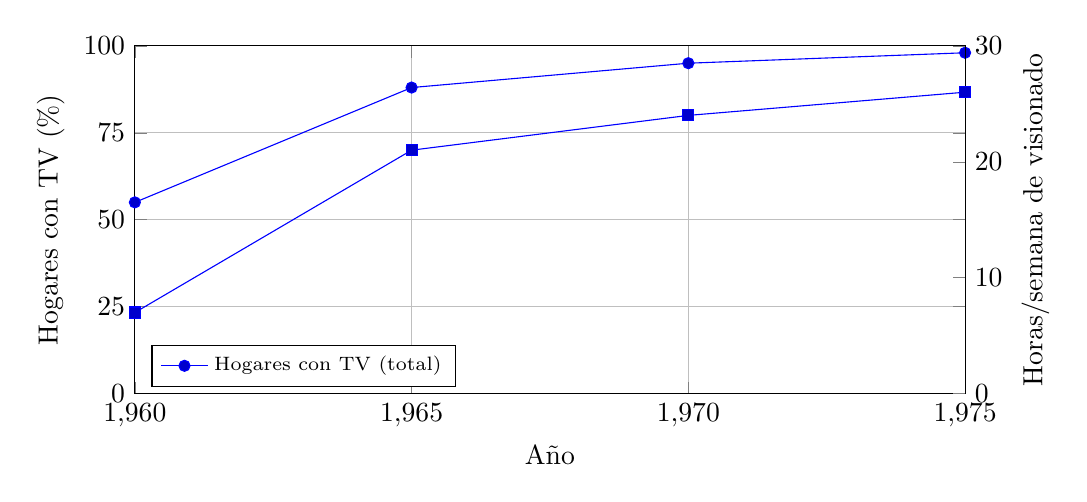
\begin{tikzpicture}
		\begin{axis}[
			width=\linewidth,
			height=6cm,
			xmin=1960, xmax=1975,
			ymin=0, ymax=100,
			xlabel={Año},
			ylabel={Hogares con TV (\%)},
			xtick={1960,1965,1970,1975},
			ytick={0,25,50,75,100},
			grid=both,
			legend style={at={(0.02,0.02)},anchor=south west,font=\scriptsize},
			]
			\addplot+[mark=*] coordinates {
				(1960,55)
				(1965,88)
				(1970,95)
				(1975,98)
			};
			\addlegendentry{Hogares con TV (total)}
		\end{axis}
		\begin{axis}[
			width=\linewidth,
			height=6cm,
			xmin=1960, xmax=1975,
			ymin=0, ymax=30,
			axis y line*=right,
			axis x line=none,
			ylabel={Horas/semana de visionado},
			ytick={0,10,20,30},
			]
			\addplot+[mark=square*] coordinates {
				(1960,7)
				(1965,21)
				(1970,24)
				(1975,26)
			};
		\end{axis}
	\end{tikzpicture}
	\caption{Penetración televisiva y tiempo medio de visionado semanal en Japón (1960--1975). Valores aproximados a partir de encuestas de NHK.}
	\label{fig:japan_tv_usage}
\end{figure}

Este contexto ayuda a entender por qué \textit{Hausu} se percibe, incluso hoy, como una película ``televisiva'' en su textura: está pensada para un público acostumbrado a la intensidad visual y al zapping interno de la programación.

% =========================================================
\subsection{Cultura pop, manga y estética híbrida}
% =========================================================

La cultura pop japonesa de los sesenta y setenta estuvo profundamente influenciada por la expansión del manga comercial, la circulación de imaginarios pop internacionales y el auge de la música juvenil. El manga se consolidó como medio masivo: las tiradas de revistas \emph{shōnen} y \emph{shōjo} crecieron de forma espectacular durante los sesenta y setenta, con \emph{Weekly Shōnen Jump} alcanzando tiradas de varios millones de ejemplares a mediados de los setenta, mientras revistas como \emph{Margaret} o \emph{Nakayoshi} articulaban la cultura de chicas.\citep{Shamoon2012,ShamoonShojoRevolution} El \emph{gekiga} ---manga de tono adulto y realista--- introdujo temas de violencia, erotismo y marginalidad que dialogaban con el cine de explotación.

Paralelamente, el \emph{pop-art} fue reinterpretado por diseñadores como Tadanori Yokoo, cuyas portadas psicodélicas y carteles cinematográficos fusionaban iconografía tradicional japonesa, imágenes publicitarias y estética \emph{sixties} occidental.\citep{YokooDesign} En la música, el movimiento \emph{Group Sounds} y posteriormente el rock japonés crearon escenas juveniles asociadas a Shinjuku y a otros barrios urbanos. Programas televisivos infantiles y de \emph{tokusatsu} ---como \emph{Ultraman} (1966)--- mezclaban acción, fantasía y merchandising, generando un ecosistema transmediático que unía juguetes, series y películas.

Obayashi se sitúa en el epicentro de esta circulación pop. Sus anuncios incorporan recursos gráficos del manga y del diseño pop; su cine tempranamente experimenta con superposiciones, collages y animación. En \textit{Hausu}, esta estética híbrida aparece en múltiples niveles:

\begin{itemize}
	\item los colores hipersaturados y los fondos ilustrados que remiten tanto a decorados teatrales como a páginas de manga coloreadas;
	\item el humor gestual, los \emph{freeze-frames} y las expresiones caricaturescas, próximos a la gramática del \emph{shōnen}/\emph{shōjo};
	\item la fragmentación del cuerpo (cabezas voladoras, miembros seccionados, gatos gigantes) que recuerda al manga de horror y a las ilustraciones de revistas juveniles;
	\item la lógica episódica y acumulativa de la narración, que funciona casi como una sucesión de \emph{chapters} de serial.
\end{itemize}

Mientras que algunos críticos han leído esta estética como simple kitsch o acumulación de recursos sin coherencia,\citep{CriticaKitschHausu} otros han señalado que precisamente esta hibridez permite a \textit{Hausu} funcionar como una especie de ``museo pop'' de la cultura visual japonesa de su tiempo, condensando en 88 minutos un archivo de estilos, modas y fantasías juveniles.\citep{McRoy2008}

Podemos representar de forma esquemática el crecimiento de la cultura impresa juvenil mediante la evolución de algunas revistas clave:

\begin{figure}[t]
	\centering
	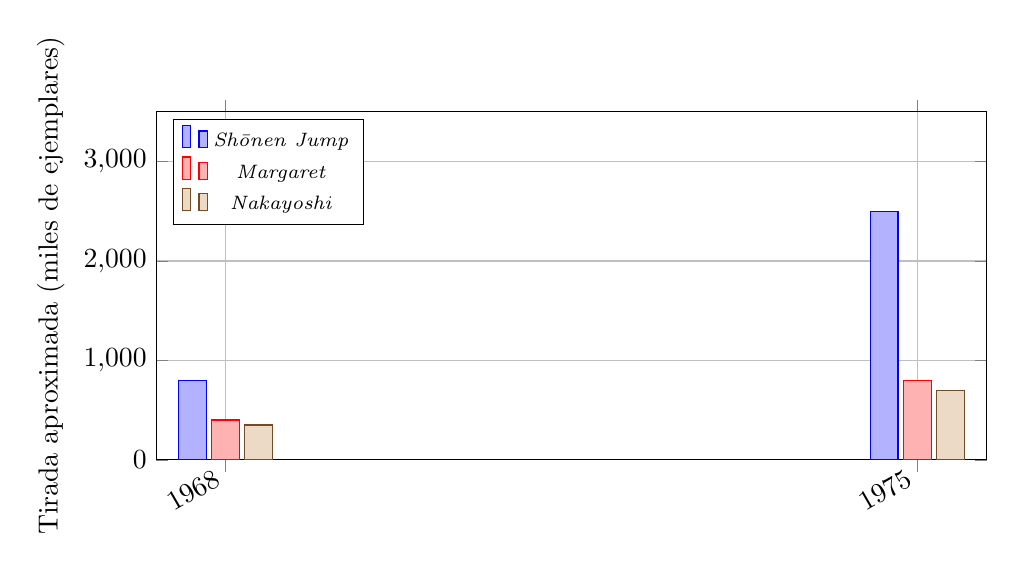
\begin{tikzpicture}
		\begin{axis}[
			ybar,
			width=\linewidth,
			height=6cm,
			bar width=10pt,
			ymin=0, ymax=3500,
			xtick=data,
			xticklabel style={rotate=30,anchor=east},
			symbolic x coords={1968,1975},
			ylabel={Tirada aproximada (miles de ejemplares)},
			legend style={at={(0.02,0.98)},anchor=north west,font=\scriptsize},
			grid=both,
			]
			\addplot coordinates {(1968,800) (1975,2500)};
			\addlegendentry{\emph{Shōnen Jump}}
			\addplot coordinates {(1968,400) (1975,800)};
			\addlegendentry{\emph{Margaret}}
			\addplot coordinates {(1968,350) (1975,700)};
			\addlegendentry{\emph{Nakayoshi}}
		\end{axis}
	\end{tikzpicture}
	\caption{Crecimiento aproximado de la tirada de revistas de manga juveniles en Japón (1968--1975). Valores indicativos a partir de estimaciones de la industria.}
	\label{fig:manga_circulation}
\end{figure}

La gráfica subraya el aumento del mercado juvenil impreso, que coexiste con televisión y cine, y que alimenta un imaginario común de personajes, situaciones y emociones del que \textit{Hausu} se nutre de forma explícita.

% =========================================================
\subsection{Movimientos artísticos y vanguardias japonesas}
% =========================================================

La década de 1960 vio el auge de movimientos artísticos radicales que redefinieron el arte japonés y su relación con la política, el cuerpo y el espacio urbano. En el ámbito cinematográfico, la \emph{Art Theatre Guild} (ATG) emergió como plataforma clave para el cine de vanguardia, distribuyendo y produciendo obras de Ōshima, Yoshida, Terayama, Adachi y otros cineastas experimentales.\citep{HarvardATG,MidnightEyeATG} Libres en gran medida de las restricciones de los estudios, estos autores exploraron estructuras narrativas fragmentarias, montaje disyuntivo, erotismo explícito y crítica frontal al Estado y al capitalismo.

Paralelamente, movimientos como el \emph{butō} (Tatsumi Hijikata, Kazuo Ohno) desarrollaron una danza de cuerpos distorsionados, movimientos mínimos y temporalidades dilatadas, en abierta oposición tanto a la danza tradicional como al ballet occidental.\citep{FraleighButoh} Grupos de arte conceptual como \emph{Hi-Red Center} llevaron a cabo intervenciones urbanas y performances que cuestionaban la higiene social, el control y la vida cotidiana en la ciudad de alta modernidad. El teatro de Terayama (\emph{Tenjō Sajiki}) mezcló circo, cabaret, \emph{happenings} y cine en espectáculos multimedia que rompían la cuarta pared y desestabilizaban al espectador.\citep{Gerow2010,SharpUnderground}

Aunque Obayashi no perteneció formalmente a ATG, sí compartió circuitos y sensibilidades con este underground. Sus cortos experimentales en 8\,mm y 16\,mm se proyectaron en espacios alternativos, y su participación en colectivos como el ``Group of Three'' junto a Takabayashi y Iimura evidencia su implicación en la escena.\citep{MakinoATG,ACCObayashi} La diferencia fundamental es que, mientras ATG tendía hacia un cine áspero, abiertamente político y muchas veces pesimista, Obayashi redirige la experimentación formal hacia un registro más lúdico, nostálgico y afectivo.

En \textit{Hausu} pueden rastrearse múltiples huellas de estas vanguardias:

\begin{itemize}
	\item el uso de sobreimpresiones, solarizaciones y trucajes ópticos recuerda al cine experimental de los sesenta;
	\item la fragmentación del cuerpo y las poses extremas de las protagonistas dialogan con ciertas estéticas del \emph{butō};
	\item la ruptura constante del realismo espacial ---habitaciones que cambian de escala, perspectivas imposibles--- conecta con las exploraciones de espacio teatral de Terayama;
	\item la frontalidad de algunas composiciones, con personajes mirando a cámara, hace visible el artificio de la representación.
\end{itemize}

Podemos representar de forma esquemática la centralidad de ATG y de los circuitos alternativos en la década:

\begin{figure}[t]
	\centering
	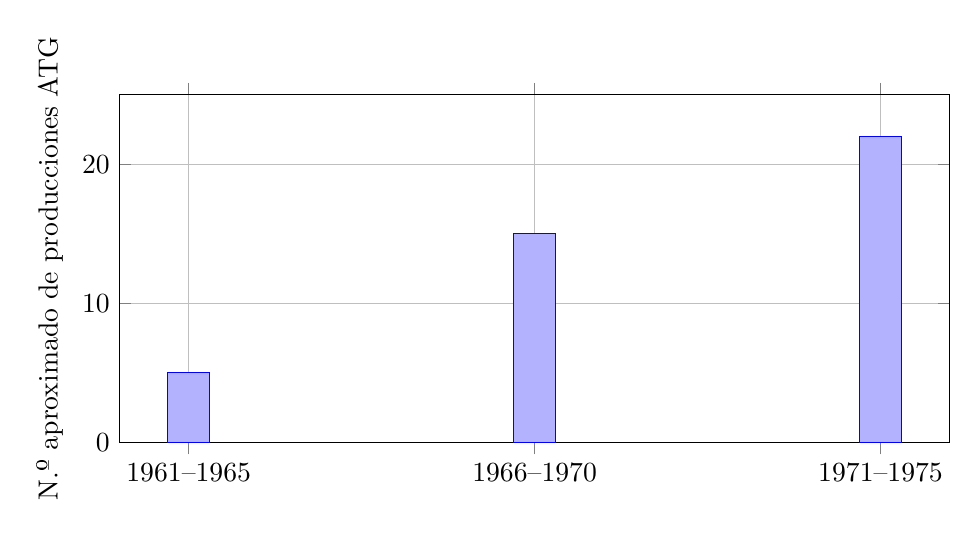
\begin{tikzpicture}
		\begin{axis}[
			ybar,
			width=\linewidth,
			height=6cm,
			bar width=15pt,
			ymin=0, ymax=25,
			xtick=data,
			symbolic x coords={1961--1965,1966--1970,1971--1975},
			ylabel={N.º aproximado de producciones ATG},
			grid=both,
			]
			\addplot coordinates { (1961--1965,5) (1966--1970,15) (1971--1975,22) };
		\end{axis}
	\end{tikzpicture}
	\caption{Crecimiento aproximado de las producciones de ATG (1961--1975). Valores indicativos basados en recuentos de filmografías de ATG.}
	\label{fig:atg_output}
\end{figure}

Este incremento ilustra cómo, en paralelo al colapso del sistema de estudios, se consolidó una infraestructura alternativa que hizo posible la circulación de formas radicales de cine; \textit{Hausu} puede entenderse como un intento singular de introducir parte de esa radicalidad en el marco de un gran estudio como Toho.

% =========================================================
\subsection{El trauma bélico y la memoria generacional}
% =========================================================

Aunque la cultura pop y juvenil domina la superficie de la época, la memoria de la guerra sigue siendo un elemento central en la identidad japonesa de posguerra. Trabajos como los de \citeauthor{Igarashi2000} y \citeauthor{Seaton2007} han subrayado que las memorias de la guerra en Japón están lejos de ser unívocas: se trata de un campo de disputa entre discursos victimistas, narrativas críticas del militarismo, revisionismos nacionalistas y silencios estructurales.\citep{Igarashi2000,Seaton2007,Penney2024}

En el terreno del cine, la posguerra temprana generó obras de duelo y reconstrucción (\emph{Children of Hiroshima}, Shindō, 1952; \emph{Hiroshima}, Sekigawa, 1953), mientras que los años sesenta y setenta vieron un retorno crítico a la guerra en películas de Okamoto (\emph{Japan's Longest Day}, 1967), Ichikawa (\emph{The Burmese Harp}, 1956; \emph{Fires on the Plain}, 1959) o Imamura (\emph{Black Rain}, 1989, ligeramente posterior pero heredera de estas preocupaciones).\citep{Penney2024,CoatesWarCinema} La televisión, por su parte, contribuyó a institucionalizar memorias victimizantes mediante dramas de prestigio emitidos en fechas conmemorativas.

Obayashi, originario de la prefectura de Hiroshima y niño durante la guerra, incorpora esta dimensión de manera personal y persistente. Como han señalado diversos estudios, su obra está atravesada por una reflexión sobre la infancia, la pérdida y la destrucción nuclear, que se hace explícita en películas posteriores como \emph{The Little Girl Who Conquered Time} (1983) o su trilogía antibélica tardía, pero que ya está presente en la imaginería fantasmática de \textit{Hausu}.\citep{McRoy2008,ObayashiHiroshimaInterview}

En \textit{Hausu}, la tía que espera eternamente a un prometido muerto en la guerra funciona como metáfora de un país atrapado entre trauma y modernización. La casa misma puede leerse como una encarnación espacial del trauma: devora cuerpos jóvenes, absorbe vidas futuras, rehusándose a abandonar el pasado. La oposición entre las protagonistas ---jóvenes, vitales, asociadas a la cultura pop--- y la tía espectral ---atemporal, congelada en el recuerdo de la guerra--- condensa una tensión generacional que ha sido descrita también en otros textos culturales de la época.\citep{Penney2024}

Para situar \textit{Hausu} dentro de esta cartografía de memoria, resulta útil un breve esquema cronológico de algunas obras y acontecimientos clave:

\begin{figure}[t]
	\centering
	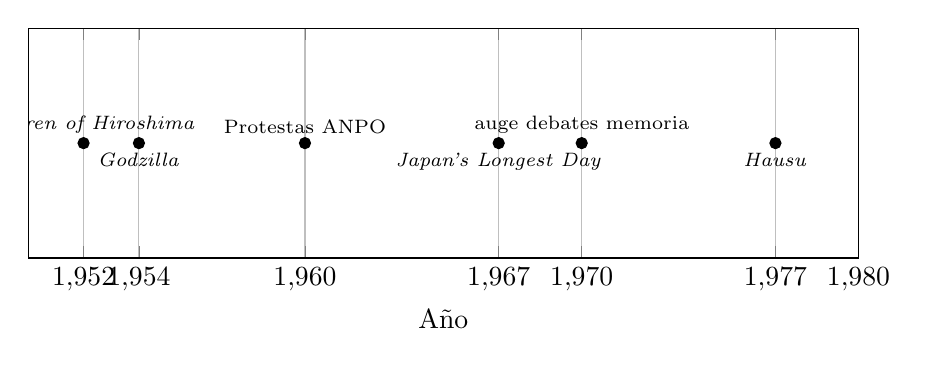
\begin{tikzpicture}
		\begin{axis}[
			width=\linewidth,
			height=4.5cm,
			ymin=0, ymax=1,
			xmin=1950, xmax=1980,
			ytick=\empty,
			xtick={1952,1954,1960,1967,1970,1977,1980},
			xlabel={Año},
			grid=both,
			]
			\addplot[only marks,mark=*] coordinates {
				(1952,0.5) % Children of Hiroshima
				(1954,0.5) % Godzilla
				(1960,0.5) % Anpo protests
				(1967,0.5) % Japan's Longest Day
				(1970,0.5) % retorno memoria
				(1977,0.5) % Hausu
			};
			\node[anchor=south] at (axis cs:1952,0.5) {\scriptsize \emph{Children of Hiroshima}};
			\node[anchor=north] at (axis cs:1954,0.5) {\scriptsize \emph{Godzilla}};
			\node[anchor=south] at (axis cs:1960,0.5) {\scriptsize Protestas ANPO};
			\node[anchor=north] at (axis cs:1967,0.5) {\scriptsize \emph{Japan's Longest Day}};
			\node[anchor=south] at (axis cs:1970,0.5) {\scriptsize auge debates memoria};
			\node[anchor=north] at (axis cs:1977,0.5) {\scriptsize \emph{Hausu}};
		\end{axis}
	\end{tikzpicture}
	\caption{Esquema de algunos hitos en la construcción de la memoria bélica en el cine y la cultura japonesa.}
	\label{fig:war_memory_timeline}
\end{figure}

Este esquema sitúa a \textit{Hausu} en un punto intermedio: no es un drama bélico explícito, pero sí un film que desplaza el trauma a un registro fantástico-pop, haciendo que el horror de la guerra se manifieste bajo la forma de una casa voraz que devora a la juventud.

% =========================================================
\subsection{Síntesis: fuerzas culturales que confluyen en \emph{Hausu}}
% =========================================================

\emph{Hausu} se sitúa en el cruce de todas las fuerzas descritas:

\begin{enumerate}
	\item \textbf{Juventud como sujeto visual}: las siete protagonistas encarnan arquetipos pop diseñados para el público adolescente, en sintonía con la mercantilización de la juventud y con la centralidad de estudiantes y colegialas en el imaginario de la época.
	\item \textbf{Televisión y publicidad}: el film adopta la estética rápida, saturada y antinatural de la TV comercial y del \emph{CM}, poniendo en primer plano trucajes visuales, superposiciones y cortinillas gráficas.
	\item \textbf{Cultura pop y manga}: la exageración visual, la lógica episódica y la fragmentación del cuerpo remiten a lenguajes del manga y de programas infantiles de \emph{tokusatsu}, filtrados por la sensibilidad pop-art.
	\item \textbf{Vanguardias japonesas}: la fragmentación de la narración, el collage de estilos y el anti-realismo dialogan con el cine de ATG, el \emph{butō} y el teatro de Terayama, pero traducidos a un registro accesible y lúdico.
	\item \textbf{Memoria bélica}: la tía espectral y la casa como espacio traumático conectan la trama de terror con la herida histórica de la guerra y la hibridez generacional de la posguerra tardía.
\end{enumerate}

Lejos de ser un producto excéntrico y aislado, \emph{Hausu} funciona como una condensación estética de un Japón en plena transformación cultural: entre televisión y memoria, entre modernización y nostalgia, entre juventud y trauma, entre vanguardia y espectáculo. Su singularidad reside precisamente en la capacidad de articular, en un único dispositivo cinematográfico, los lenguajes fragmentarios de la publicidad televisiva, los imaginarios del manga adolescente, las exploraciones formales de la vanguardia y los fantasmas persistentes de la guerra.

Podemos visualizar esta convergencia mediante un diagrama conceptual:

\begin{figure}[t]
	\centering
	\begin{tikzpicture}[node distance=1.8cm]
		\node[draw, rounded corners, align=center, thick] (hausu) {\textbf{\emph{Hausu} (1977)}\\Film híbrido juvenil-pop};
		\node[draw, rounded corners, above left=of hausu, align=center] (youth) {Juventud\\modernización\\urbana};
		\node[draw, rounded corners, above right=of hausu, align=center] (tv) {Televisión\\y publicidad};
		\node[draw, rounded corners, below left=of hausu, align=center] (pop) {Cultura pop\\manga / anime};
		\node[draw, rounded corners, below right=of hausu, align=center] (avant) {Vanguardias\\ATG, butō, teatro};
		\node[draw, rounded corners, below=3.2cm of hausu, align=center] (war) {Memoria bélica\\trauma Hiroshima};
		
		\draw[->, thick] (youth) -- (hausu);
		\draw[->, thick] (tv) -- (hausu);
		\draw[->, thick] (pop) -- (hausu);
		\draw[->, thick] (avant) -- (hausu);
		\draw[->, thick] (war) -- (hausu);
	\end{tikzpicture}
	\caption{Esquema conceptual de las fuerzas culturales y mediáticas que confluyen en \emph{Hausu}.}
	\label{fig:hausu_forces_network}
\end{figure}

Este esquema sintetiza la tesis central del capítulo: \textit{Hausu} no es únicamente una rareza de culto, sino un nodo donde se cruzan tendencias industriales, mediáticas y culturales del Japón de 1965--1977.

% =========================================================
\subsection{Conclusión}
% =========================================================

El Japón de 1965--1977 fue un laboratorio cultural donde convergieron modernización acelerada, masificación televisiva, experimentación artística y redefinición de lo juvenil. La rápida expansión económica y urbana generó nuevas formas de subjetividad y consumo; la televisión y la publicidad reconfiguraron el régimen de imágenes y la economía de la atención; el manga y la cultura pop produjeron imaginarios híbridos de género, cuerpo y deseo; las vanguardias cinematográficas y performativas cuestionaron los límites entre arte y política; y la memoria de la guerra se debatió entre silencios, revisiones críticas y fantasmas persistentes.

Nobuhiko Obayashi, situado en medio de esas fuerzas, desarrolló una poética visual única: lúdica y crítica, pop y melancólica, artesanal y tecnológica. \emph{Hausu} cristaliza de forma particularmente intensa esta poética, funcionando como archivo emocional de la posguerra japonesa y como puente entre vanguardia experimental y cultura popular. Comprender las fuerzas culturales y mediáticas que aquí se han analizado resulta esencial para interpretar no sólo \emph{Hausu}, sino el conjunto de la obra de Obayashi y, más ampliamente, las mutaciones del cine japonés tardomoderno.
